\chapter{Primfaktorzerlegung}

Es gilt der Fundamentalsatz der Arithmetik: Jede positive ganze Zahl lässt sich als Produkt von Primzahlen darstellen, und diese Darstellung ist bis auf die Reihenfolge der Primzahlen eindeutig\cite{scala}. 
Diese Primzahlen nennt man die Primfaktoren der Zahl. 
Man kennt bisher keine Methode, um die Primfaktorzerlegung einer beliebigen gegebenen Zahl effizient zu bestimmen, d. h. in einer Zeit, die polynomiell mit der Länge der Zahl wächst. 
Die Faktorisierungsannahme besagt, dass es eine solche Methode auch nicht gibt. 
Man versucht, die Zeit mit geeigneten Faktorisierungsverfahren zu minimieren.

Aufgrund dieses Satzes, also dass sich jede natürliche Zahl größer 0 durch Multiplikation von Primzahlen eindeutig darstellen lässt, nehmen die Primzahlen eine besondere atomare Stellung in der Mathematik ein\cite{rltl}.
Alexander K. Dewdney bezeichnete diese als den Elementen der Chemie weitgehend ähnlich.

In \vref{fig:tolleAbbildung} sehen Sie eine schematische Darstellung der Primfaktorzerlegung.

\begin{figure}[h]
    \centering
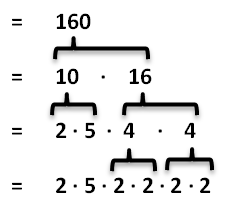
\includegraphics[width=0.5\linewidth]{primeFac.png}

    \caption{Eine super Abbildung}
    \label{fig:tolleAbbildung}
\end{figure}

